\subsection{Configurazione del panel G\&B}
Una volta aggiunto il panel alla dashboard, per poterlo configurare è necessario accedere all'area di editing del panel:
\begin{enumerate}
	\item Cliccare sul nome del panel;
	\item Nel menu dropdown, selezionare "\textit{Edit}".
\end{enumerate}
oppure:
\begin{enumerate}
	\item Cliccare sul panel;
	\item Premere il tasto "\textit{E}".
\end{enumerate}
\begin{figure} [H]
	\centering
	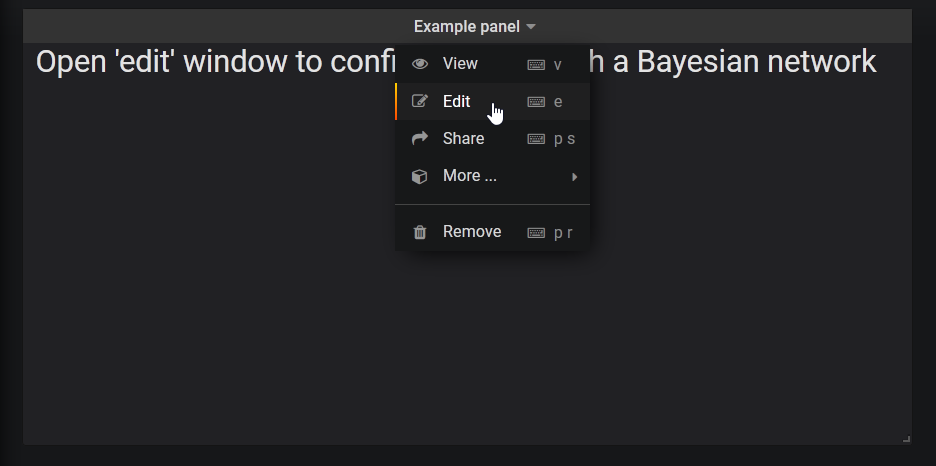
\includegraphics[scale=0.55]{Img/editmode} 
	\caption{Menu dropdown in cui selezionare "\textit{Edit}"} \label{} 
\end{figure} 
Comparirà l'area di editing, che permette di modificare le informazioni di base del panel e di configurarlo con una rete Bayesiana.
\begin{figure} [H]
	\centering
	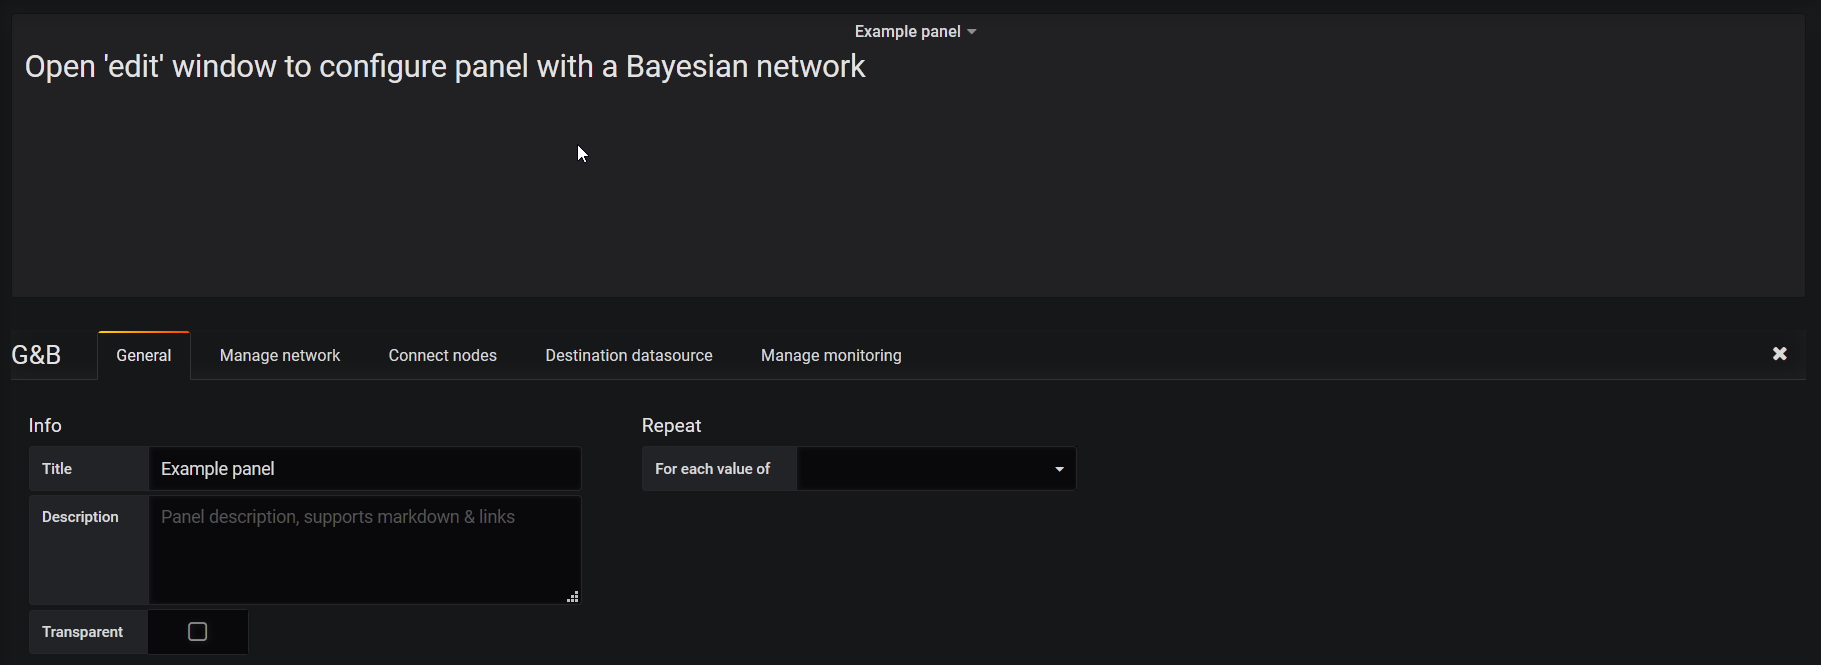
\includegraphics[scale=0.4]{Img/editview} 
	\caption{Area di editing} \label{} 
\end{figure} 
\subsubsection{Caricamento, modifica e download di una rete}
Nell'area di editing, selezionare la tab "\textit{Manage network}".
\begin{figure} [H]
	\centering
	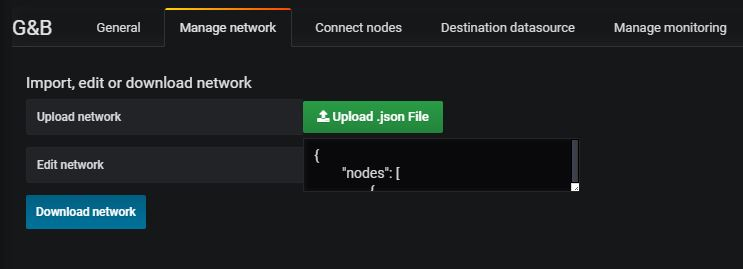
\includegraphics[scale=0.55]{Img/managenet} 
	\caption{Tab di gestione della rete} \label{} 
\end{figure} 
In questa tab è possibile eseguire tre operazioni: caricare una rete Bayesiana, modificare quella in utilizzo oppure scaricarla sotto forma di file JSON.
\paragraph{Caricamento di una rete Bayesiana}~\\
	Per caricare una nuova rete Bayesiana, è sufficiente cliccare sul pulsante "\textit{Upload .json File}" e selezionare il file contenente la rete desiderata. Al momento sono supportati solo i file JSON.
\paragraph{Modifica di una rete Bayesiana}~\\
	Una volta caricata con successo, sarà possibile visualizzare e modificare la rete all'interno di un'apposita casella di testo, contrassegnata dall'etichetta "\textit{Edit network}"; le modifiche vengono applicate in modo istantaneo. Per evitare malfunzionamenti, assicurarsi che le modifiche rispettino la struttura della rete descritta in §4.
\paragraph{Download di una rete Bayesiana}~\\
	Infine, premendo il bottone "\textit{Download network}", è possibile scaricare la rete Bayesiana in utilizzo (comprese eventuali modifiche) sotto forma di file JSON.